% \date{May 14, 2024}
% \author{Deralive / Shichien}
% \title{华东师范大学软件学院实验报告模板}
% 注意事项:编译两次,以确保目录、页码完整显示
% 模板文件:https://github.com/Shichien/ECNU-LateX-Template

\def\allfiles{}

%————————————多文件编译————————————%
% \ifx\allfiles\undefined
% 	    \begin{document}
% \else
% \fi

% Content

% \ifx\allfiles\undefined
% 	    \end{document}
% 	\else
% 	\fi
%—————————————————————————————————%

\documentclass[14pt,a4paper,UTF8,twoside]{article}

\usepackage{amsmath}
\usepackage{graphicx}
\usepackage{geometry} 
\usepackage{ctex}
\usepackage{booktabs} % 表格库
\usepackage{titlesec} % 标题库
\usepackage{fancyhdr} % 页眉页脚库
\usepackage{lastpage} % 页码数库
\usepackage{listings} % 代码块包
\usepackage{xcolor}
\usepackage[hidelinks]{hyperref}
\usepackage{tikz}
\usepackage{tikz-qtree}
\usepackage{fontspec} % 允许设置字体
\usepackage{unicode-math} % 允许数学公式使用特定字体
\usepackage{mwe}
\usepackage{zhlipsum} % 中文乱数文本
\usepackage{amsmath}
\usepackage{amsfonts}
\usepackage{enumitem}
\usepackage{xcolor}
\usepackage{float} % 浮动体环境
\usepackage{subcaption} % 子图包
\usepackage{biblatex}
\addbibresource{references.bib} % 指定你的.bib文件名称

\definecolor{mygreen}{rgb}{0,0.6,0}
\definecolor{mygray}{rgb}{0.5,0.5,0.5}
\definecolor{mymauve}{rgb}{0.58,0,0.82}

\date{} % 留空,以让编译时去除日期

%———————————————注意事项—————————————————%

% 1、如果编译显示失败,但没有错误信息,就是 filename.pdf 正在被占用
% 2、在文件夹中的终端使用 Windows > xelatex filename.tex 也可编译

%—————————————华东师范大学———————————————%

% 论文制作时须加页眉,页眉从中文摘要开始至论文末
% 偶数页码内容为:华东师范大学硕士学位论文,奇数页码内容为学位论文题目

%————————定义 \section 的标题样式————————%

% 注意:\chapter 等命令,内部使用的是 \thispagestyle{plain} 的排版格式
% 若需要自己加上页眉,实际是在用 \thispagestyle{fancy} 的排版格式
% 加上下面这一段指令,就能够让 \section 也使用 fancy 的排版格式
% 本质就是让目录、第一页也能够显示页眉、页脚

\fancypagestyle{plain}{
  \pagestyle{fancy}
}

\title{华东师范大学软件学院课程项目报告 - 附件} % 模板
\titleformat{\section}
    {\normalfont\bfseries\Large} % 字体大小、字体系列(\bfseries 为加粗)
    {\thesection}{1em}{}

% 设置章节的中文格式
\renewcommand\thesection{\chinese{section} \hspace{0pt}}
\renewcommand\thesubsection{\arabic{subsection} \hspace{0pt}}
% \renewcommand\thesubsubsection{\alph{subsubsection} \hspace{0pt}} % 字母编号
% \hspace{0pt} 是为了确保在章节编号和章节题目之间不要有空格,使得排版更为美观
    
%—————————————页面基础设置———————————————%

\geometry{left=10mm, right=10mm, top=20mm, bottom=20mm}

%————————————设置页眉、页脚——————————————%

\pagestyle{fancy} % 设置 plain style 的属性

% 设置页眉

\fancyhead[RE]{\footnotesize \leftmark} % Right Even 偶数页右侧显示章名 \leftmark 最高级别章名
\fancyhead[LO]{\footnotesize \rightmark} % Left Odd 奇数页左侧显示节名 \rightmark 第二级别节名
\fancyhead[C]{华东师范大学软件学院课程项目报告 - 附件} % Center 居中显示
\fancyhead[LE,RO]{~\thepage~} % 在偶数页的左侧,奇数页的右侧显示页码
\renewcommand{\headrulewidth}{1.2pt} % 页眉与正文之间的水平线粗细

% 设置页脚:在每页的右下脚以斜体显示书名

\fancyfoot[RO,RE]{\it Lab Report By \LaTeX} % 使用意大利斜体显示
\renewcommand{\footrulewidth}{0.5pt} % 页脚水平线宽度

% 设置页码:在底部居中显示页码

\pagestyle{fancy}
\fancyfoot[C]{\kaishu 第 \thepage 页 \ 共 \pageref{LastPage} 页} % LastPage 需要二次编译以获取总页数

%——————————————代码块设置———————————————%

\lstset {
    backgroundcolor=\color{white},   % choose the background color; you must add \usepackage{color} or \usepackage{xcolor}
    basicstyle=\footnotesize,        % the size of the fonts that are used for the code
    breakatwhitespace=false,         % sets if automatic breaks should only happen at whitespace
    breaklines=true,                 % sets automatic line breaking
    captionpos=bl,                   % sets the caption-position to bottom
    commentstyle=\color{mygreen},    % comment style
    deletekeywords={...},            % if you want to delete keywords from the given language
    escapeinside={\%*}{*},           % if you want to add LaTeX within your code
    extendedchars=true,              % lets you use non-ASCII characters; for 8-bits encodings only, does not work with UTF-8
    frame=single,                    % adds a frame around the code
    keepspaces=true,                 % keeps spaces in text, useful for keeping indentation of code (possibly needs columns=flexible)
    keywordstyle=\color{blue},       % keyword style
    % language=Python,               % the language of the code
    morekeywords={*,...},            % if you want to add more keywords to the set
    numbers=left,                    % where to put the line-numbers; possible values are (none, left, right)
    numbersep=5pt,                   % how far the line-numbers are from the code
    numberstyle=\tiny\color{mygray}, % the style that is used for the line-numbers
    rulecolor=\color{black},         % if not set, the frame-color may be changed on line-breaks within not-black text (e.g. comments (green here))
    showspaces=false,                % show spaces everywhere adding particular underscores; it overrides 'showstringspaces'
    showstringspaces=false,          % underline spaces within strings only
    showtabs=false,                  % show tabs within strings adding particular underscores
    stepnumber=1,                    % the step between two line-numbers. If it's 1, each line will be numbered
    stringstyle=\color{orange},      % string literal style
    tabsize=2,                       % sets default tabsize to 2 spaces
    % title=Python Code              % show the filename of files included with \lstinputlisting; also try caption instead of title
}

% 注释掉的部分用于后续插入代码,参数可调整,格式如下:

% 1、直接插入
% \begin{lstlisting}[language = ? , title = { ? } ]
%       Your code here.
% \end{lstlisting}

% 2、文件插入
% \lstinputlisting[language = C , title = ?.c] {filename.c}

%———————————————字体设置————————————————%

% \setCJKmainfont{SimSun} % 设置正文罗马族的 CJK 字体
% \renewcommand{\normalsize}{\fontsize{12pt}{15pt}\selectfont} % 设置正文字号
\linespread{1.2}

%———————————————超链接设置——————————————%

\hypersetup{
    pdfstartview=FitH, % 设置PDF文档打开时的初始视图为页面宽度适应窗口宽度(即页面水平适应)
    CJKbookmarks=true, % 用对CJK(中文、日文、韩文)字符的书签支持,确保这些字符在书签中正确显示
    bookmarksnumbered=true, % 书签带有章节编号。这对有章节编号的文档很有用
    bookmarksopen=true, % 文档打开时,书签树是展开的,方便查看所有书签
    colorlinks, % 启用彩色链接。这样,链接在PDF中会显示为彩色,而不是默认的方框
    pdfborder=001, % 设置PDF文档中链接的边框样式。001 表示链接周围没有边框,仅在单击时显示一个矩形
    linkcolor=blue, % 设置文档内部链接(如目录中的章节链接)的颜色为蓝色
    anchorcolor=blue, % 设置锚点链接(即目标在同一文档内的链接)的颜色为蓝色
    citecolor=blue, % 设置引用(如文献引用)的颜色为蓝色
}

%——————————————导言区结束,进入正文部分———————————————%

%——————————————————————————————————————%

\begin{document}

\maketitle

\begin{center} % \extracolsep{\fill} 拉伸到页面最大宽度前,保证居中显示

    \begin{tabular*}{\textwidth}{@{\extracolsep{\fill}} l  l  l }
        \hline
        课程名称:创客实践 & 成绩:\\
        姓名:张梓卫 & 学号:10235101526\\
        指导老师:陈闻杰 & 日期:2024/8/10\\
        项目名称:基于LLM的\textit{ESP32}智能设备多功能控制系统 & 班级:软工3班\\
        \hline
    \end{tabular*}

\end{center}

\tableofcontents % 目录也需要二次编译

\section{项目附加文件}
\begin{itemize}
    \item \textbf{partitions.csv} - 用于ESP32中Flash分区配置,存储程序、数据、参数等。
    \item \textbf{src} - 源代码目录,包含项目的源代码。
    \item \textbf{configuration.h} - 项目配置文件,包含项目的常量、宏定义、Wi-Fi设置等。
    \item \textbf{include} - 头文件目录,包含项目的头文件。
    \item \textbf{lib} - 库文件目录,包含项目的库文件。
\end{itemize}

\section{ESP-Wroom-32}

\begin{figure} [H]
    \centering
    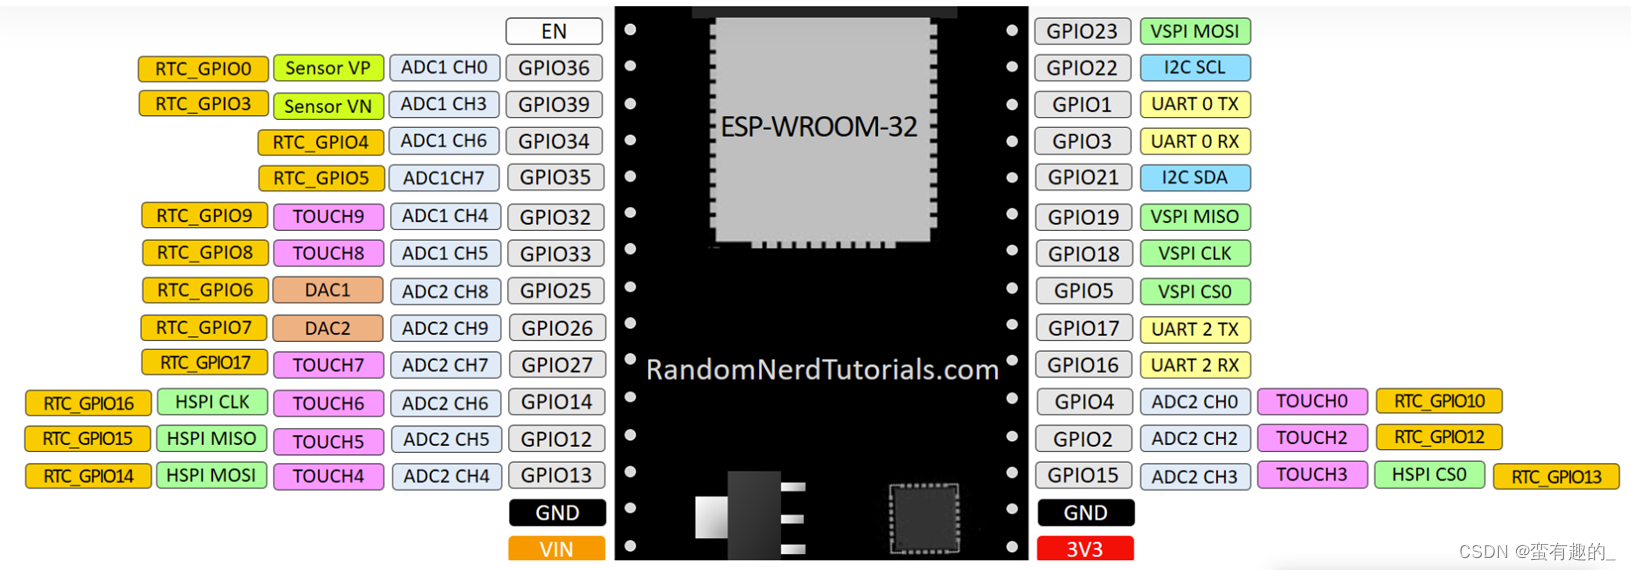
\includegraphics[width=0.8\textwidth]{../img/ESPWroom.png}
    \caption{ESP-Wroom-32}
\end{figure}
\section{MAX98357A}

\begin{figure} [H]
    \centering
    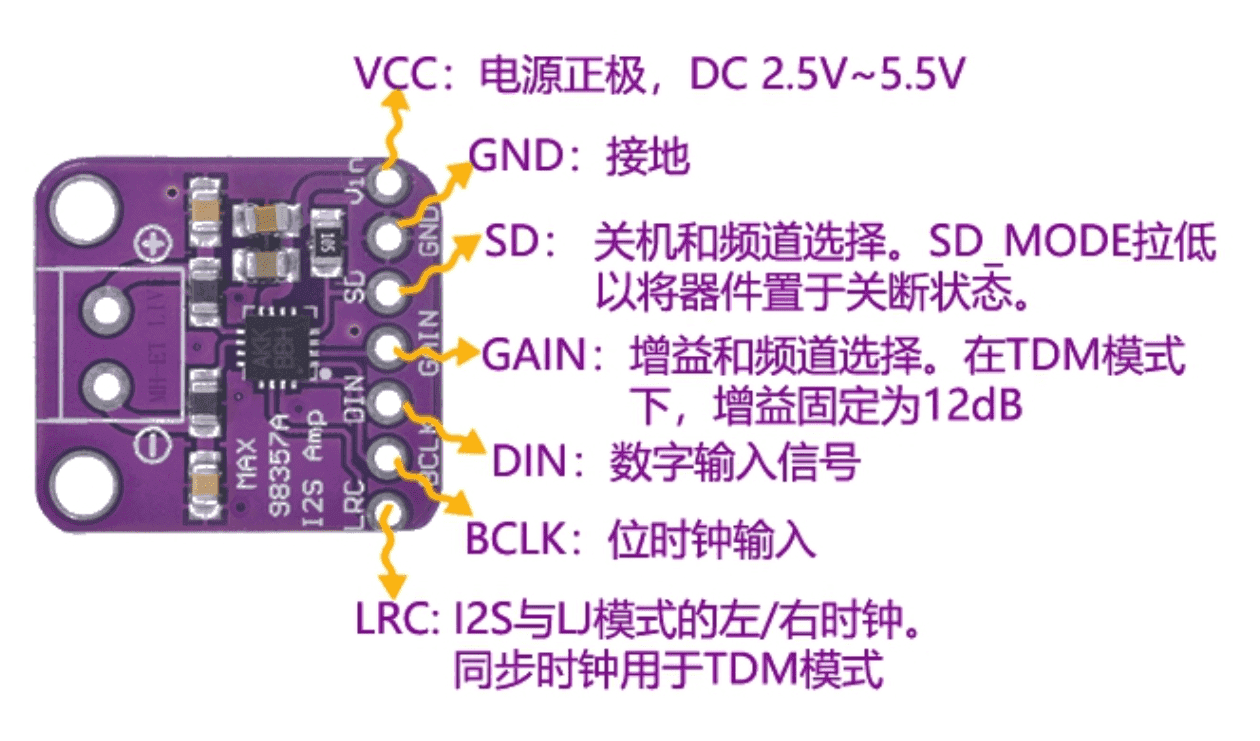
\includegraphics[width=0.4\textwidth]{../img/MAX98357A.png}
    \caption{MAX98357A}
\end{figure}

\begin{table} [H]
    \centering
    \begin{tabular}{|c|c|}
        \hline
        \textbf{MAX98357A模块引脚} & \textbf{引脚说明}                \\ \hline
        VIN                    & 电源正(2.5V-5.5V)               \\ \hline
        GND                    & 电源地                          \\ \hline
        SD                     & 关机和频道选择。SD MODE拉低以将器件处于关断状态。 \\ \hline
        GAIN                   & 增益和频道选择。在TDM模式下,增益固定为12dB    \\ \hline
        DIN                    & 数字信号输入                       \\ \hline
        BCLK                   & 位时钟输入                        \\ \hline
        LRC                    & I2S与LJ模式的左/右时钟。同步时钟用于TDM模式   \\ \hline
    \end{tabular}
    \caption{MAX98357A模块引脚说明}
\end{table}

\section{INMP441 MEMS}

\begin{figure} [H]
    \centering
    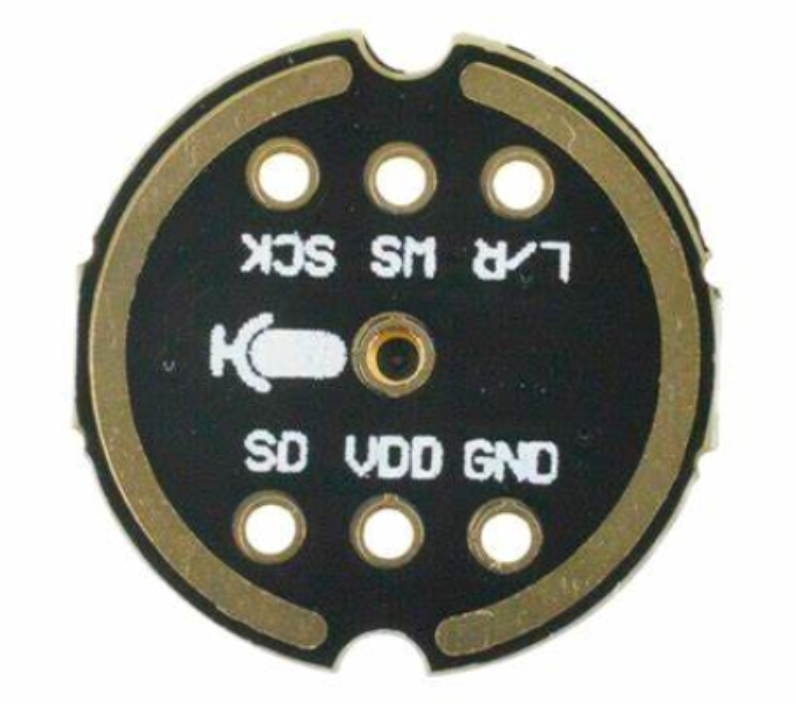
\includegraphics[width=0.2\textwidth]{../img/INMP441.png}
    \caption{INMP441 Mems}
\end{figure}

\begin{table} [H]
    \centering
    \begin{tabular}{|c|p{15cm}|}
        \hline
        \textbf{信号} & \textbf{描述}                                                                                           \\ \hline
        SCK         & I2S时钟线,是由主机产生的高频方波,用来控制每位数据的传输时序                                                                      \\ \hline
        SD          & I2S数据线,从机通过这根线把ADC采样值发送给主机                                                                            \\ \hline
        WS          & I2S声道选择线,I2S协议可以传输左右两个声道的数据,WS信号是由主机发送给从机的,从机根据WS的电平高低,判断当前数据帧发送左声道还是右声道数据。WS低电平时,从机发送左声道数据,高电平发送右声道。 \\ \hline
        L/R         & 芯片左右声道选择线,每个麦克风只能检测一处声源,因此若要进行双声道录音,就要使用两个模块,一左一右放置。                                                  \\ \hline
    \end{tabular}
    \caption{I2S信号线说明}
\end{table}

\section{MPU6050 六轴传感器}

MPU6050由具有微机电系统(MEMS)技术的三轴陀螺仪组成。

\begin{figure} [H]
    \centering
    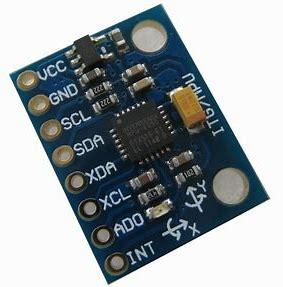
\includegraphics[width=0.2\textwidth]{../img/MPU6050.jpg}
    \caption{MPU6050}
\end{figure}


\begin{table} [H]
    \centering
    \begin{tabular}{|l|l|}
    \hline
    \textbf{参数}                     & \textbf{描述}                                \\ \hline
    芯片型号                           & MPU6050                                      \\ \hline
    加速度计范围                       & $\pm$2g, $\pm$4g, $\pm$8g, $\pm$16g          \\ \hline
    陀螺仪范围                         & $\pm$250, $\pm$500, $\pm$1000, $\pm$2000 °/s \\ \hline
    工作电压                           & 3.3V-5V                                      \\ \hline
    接口                               & I2C (400kHz) / SPI                           \\ \hline
    工作温度范围                       & -40°C 至 +85°C                                \\ \hline
    \end{tabular}
    \caption{MPU6050参数}
    \label{tab:MPU6050参数}
\end{table}

\section{MQ-135 有毒气体传感器}

MQ-135是一种空气质量传感器,用于检测空气中的一氧化碳、氮氧化物、酒精、氨气和烟雾等有害气体。
工作原理是通过化学反应来检测目标气体的浓度,并将结果转换为电信号输出。

对于需要读取不同的气体,需要设置不同的系数,系数表如下所示:

\begin{table} [H]
    \centering
    \begin{tabular}{|c|c|c|}
    \hline
    \textbf{Gas} & \textbf{a} & \textbf{b} \\
    \hline
    CO & 605.18 & -3.937 \\
    \hline
    Alcohol & 77.255 & -3.18 \\
    \hline
    CO2 & 110.47 & -2.862 \\
    \hline
    Toluen & 44.947 & -3.445 \\
    \hline
    NH4 & 102.2 & -2.473 \\
    \hline
    Aceton & 34.668 & -3.369 \\
    \hline
    Smoke & 30000000 & -8.308 \\
    \hline
    \end{tabular}
    \caption{MQ-135 系数表(来源:MQUnifiedsensor库)}
    \label{tab:MQ-135系数表}
\end{table}

\section{ESP32 Wifi Public Interfaces}

\begin{itemize}

    \item \textbf{begin()}
          \begin{itemize}
              \item 使用存储的配置连接Wi-Fi。
          \end{itemize}

    \item \textbf{disconnect(bool wifioff, bool eraseap)}
          \begin{itemize}
              \item 从当前网络断开,并可选择关闭Wi-Fi无线电或从非易失性存储中擦除AP配置。
          \end{itemize}

    \item \textbf{config(IPAddress local\_ip, IPAddress gateway, IPAddress subnet, IPAddress dns1, IPAddress dns2)}
          \begin{itemize}
              \item 配置静态IP设置,禁用DHCP。
          \end{itemize}

    \item \textbf{isConnected()}
          \begin{itemize}
              \item 如果STA接口已连接到AP,则返回\texttt{true}。
          \end{itemize}

    \item \textbf{setAutoReconnect(bool autoReconnect)}
          \begin{itemize}
              \item 启用或禁用连接丢失时的自动重连。
          \end{itemize}

    \item \textbf{getAutoReconnect()}
          \begin{itemize}
              \item 如果启用了自动重连,则返回\texttt{true}。
          \end{itemize}

    \item \textbf{waitForConnectResult(unsigned long timeoutLength)}
          \begin{itemize}
              \item 等待连接完成,返回连接状态或断开状态。
          \end{itemize}

    \item \textbf{localIP()}
          \begin{itemize}
              \item 返回STA接口的本地IP地址。
          \end{itemize}

    \item \textbf{macAddress(void)}
          \begin{itemize}
              \item 返回STA接口的MAC地址作为字符串。
          \end{itemize}

    \item \textbf{SSID() const}
          \begin{itemize}
              \item 返回连接网络的SSID。
          \end{itemize}

\end{itemize}

\section{Hmac-sha256算法}

\begin{figure} [H]
    \centering
    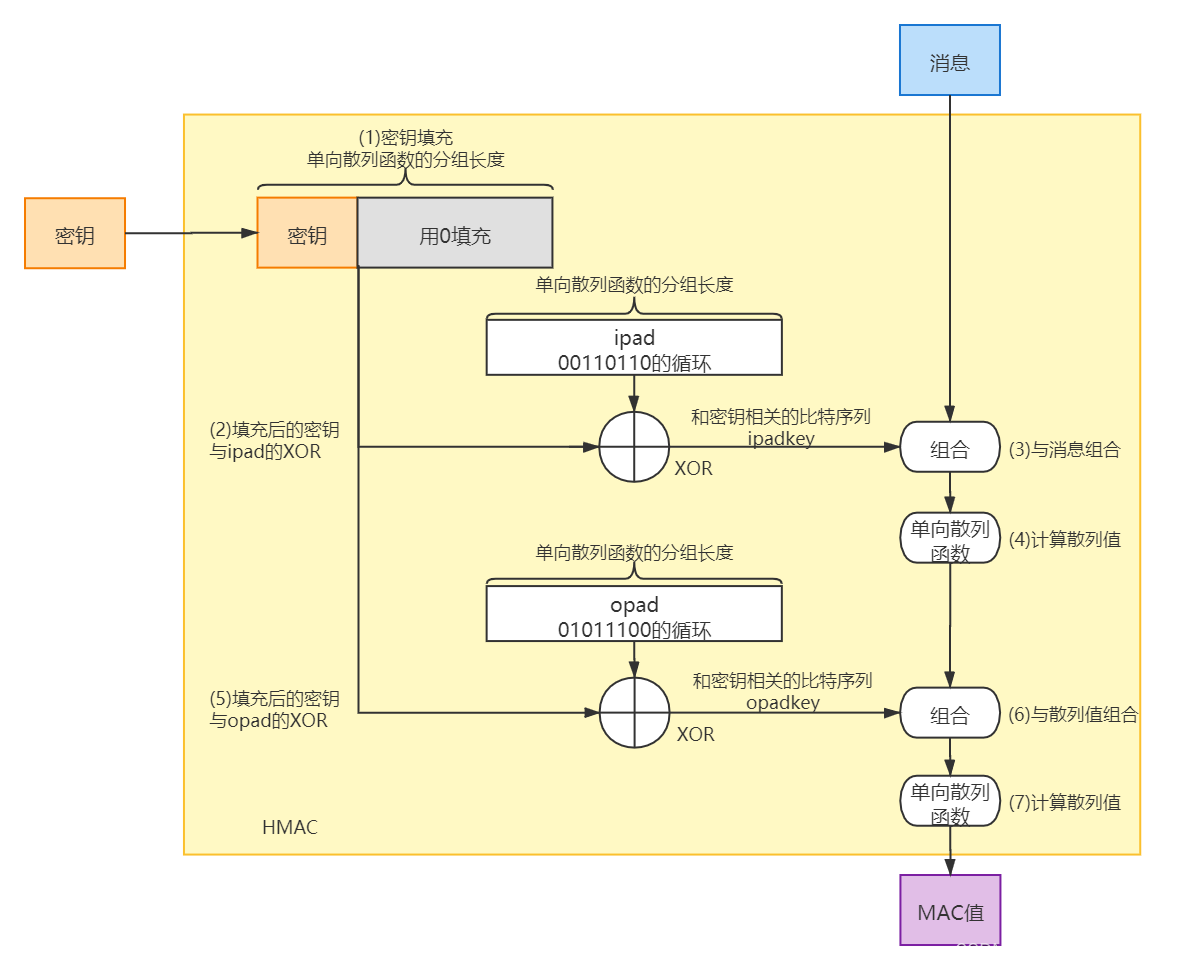
\includegraphics[width=0.6\textwidth]{../img/Hmac-sha256.png}
    \caption{Hmac-sha256算法}
    \label{fig:hmac-sha256}
\end{figure}

使用密钥 \(\text{APISecret}\) 和消息 \(\text{originalSignature}\) 计算 HMAC-SHA256:

\begin{equation}
    \text{HMAC-SHA256} = \text{HMAC}(\text{APISecret}, \text{originalSignature})
\end{equation}

其中,HMAC 的计算公式为:

\begin{equation}
    \text{HMAC}(key, message) = \text{hash}\left((key \oplus \text{opad}) \parallel \text{hash}\left((key \oplus \text{ipad}) \parallel \text{message}\right)\right)
\end{equation}

此部分内容过于复杂,我并不将重点置于此,搜索资料后发现,ESP32的核心库中已包含Mbed TLS,已帮助实现了此部分算法。

mbedTLS开源库文档:\href{https://mbed-tls.readthedocs.io/en/latest/}{\underline{https://mbed-tls.readthedocs.io/en/latest/}}

数据与哈希加密运算中,每个字节的数据都处于0-255之间,所以使用unsigned char类型来定义变量,处理字节数据。

在 Arduino 环境中使用 Mbed TLS 库进行 HMAC-SHA256 计算时,涉及的主要函数如下:

\begin{itemize}
    \item \textbf{初始化消息摘要上下文}
          \[
              \text{void mbedtls\_md\_init(mbedtls\_md\_context\_t *ctx);}
          \]
          初始化消息摘要上下文结构体。

    \item \textbf{获取消息摘要信息}
          \[
              \text{const mbedtls\_md\_info\_t *mbedtls\_md\_info\_from\_type(mbedtls\_md\_type\_t md\_type);}
          \]
          根据指定的消息摘要类型返回对应的信息结构体。

    \item \textbf{设置上下文}
          \[
              \text{int mbedtls\_md\_setup(mbedtls\_md\_context\_t *ctx, const mbedtls\_md\_info\_t *md\_info, int hmac);}
          \]
          配置消息摘要上下文,绑定指定的算法,并为 HMAC 分配资源。

    \item \textbf{开始计算}
          \[
              \text{int mbedtls\_md\_starts(mbedtls\_md\_context\_t *ctx);}
          \]
          开始消息摘要或 HMAC 计算。

    \item \textbf{输入数据}
          \[
              \text{int mbedtls\_md\_update(mbedtls\_md\_context\_t *ctx, const unsigned char *input, size\_t ilen);}
          \]
          将数据块输入到消息摘要或 HMAC 计算中,可以多次调用。

    \item \textbf{完成计算}
          \[
              \text{int mbedtls\_md\_finish(mbedtls\_md\_context\_t *ctx, unsigned char *output);}
          \]
          完成计算并将结果写入输出缓冲区。

    \item \textbf{释放资源}
          \[
              \text{void mbedtls\_md\_free(mbedtls\_md\_context\_t *ctx);}
          \]
          释放消息摘要上下文中分配的资源。
\end{itemize}

\section{引脚定义与硬件接线}

\begin{lstlisting} [language = C++]
#define RAINDROP_PIN 33
#define MQ5_PIN 36
#define MQ135_PIN 35
#define LIGHT_PIN 34
#define DHT22_PIN 25
#define FIRE_PIN 39
#define DHTTYPE DHT22
\end{lstlisting}

\subsection{主机(Master)接线表如下}

\begin{table} [H]
    \centering
    \begin{tabular}{|c|c|c|l|}
    \hline
    \textbf{引脚编号} & \textbf{引脚名称} & \textbf{接入点} & \textbf{功能/用途} \\ 
    \hline
    1  & VDD   & 3.3V & 提供3.3V电压输出 \\ 
    2  & GND   & GND  & 接地 \\ 
    3  & SD    & GPIO22 & 麦克风数据引脚 \\ 
    4  & WS    & GPIO15 & 麦克风时钟同步 \\ 
    5  & SCK   & GPIO4  & 麦克风串行时钟 \\ 
    6  & Vin   & VIN   & 音频放大模块供电 \\ 
    7  & GND   & GND   & 接地 \\ 
    8  & LRC   & GPIO27 & 音频放大模块同步信号 \\ 
    9  & BCLK  & GPIO26 & 音频放大模块时钟信号 \\ 
    10 & DIN   & GPIO25 & 音频放大模块数据输入 \\ 
    \hline
    \end{tabular}
    \caption{麦克风与音频放大模块接线引脚表}
\end{table}

\begin{figure} [H]
    \centering
    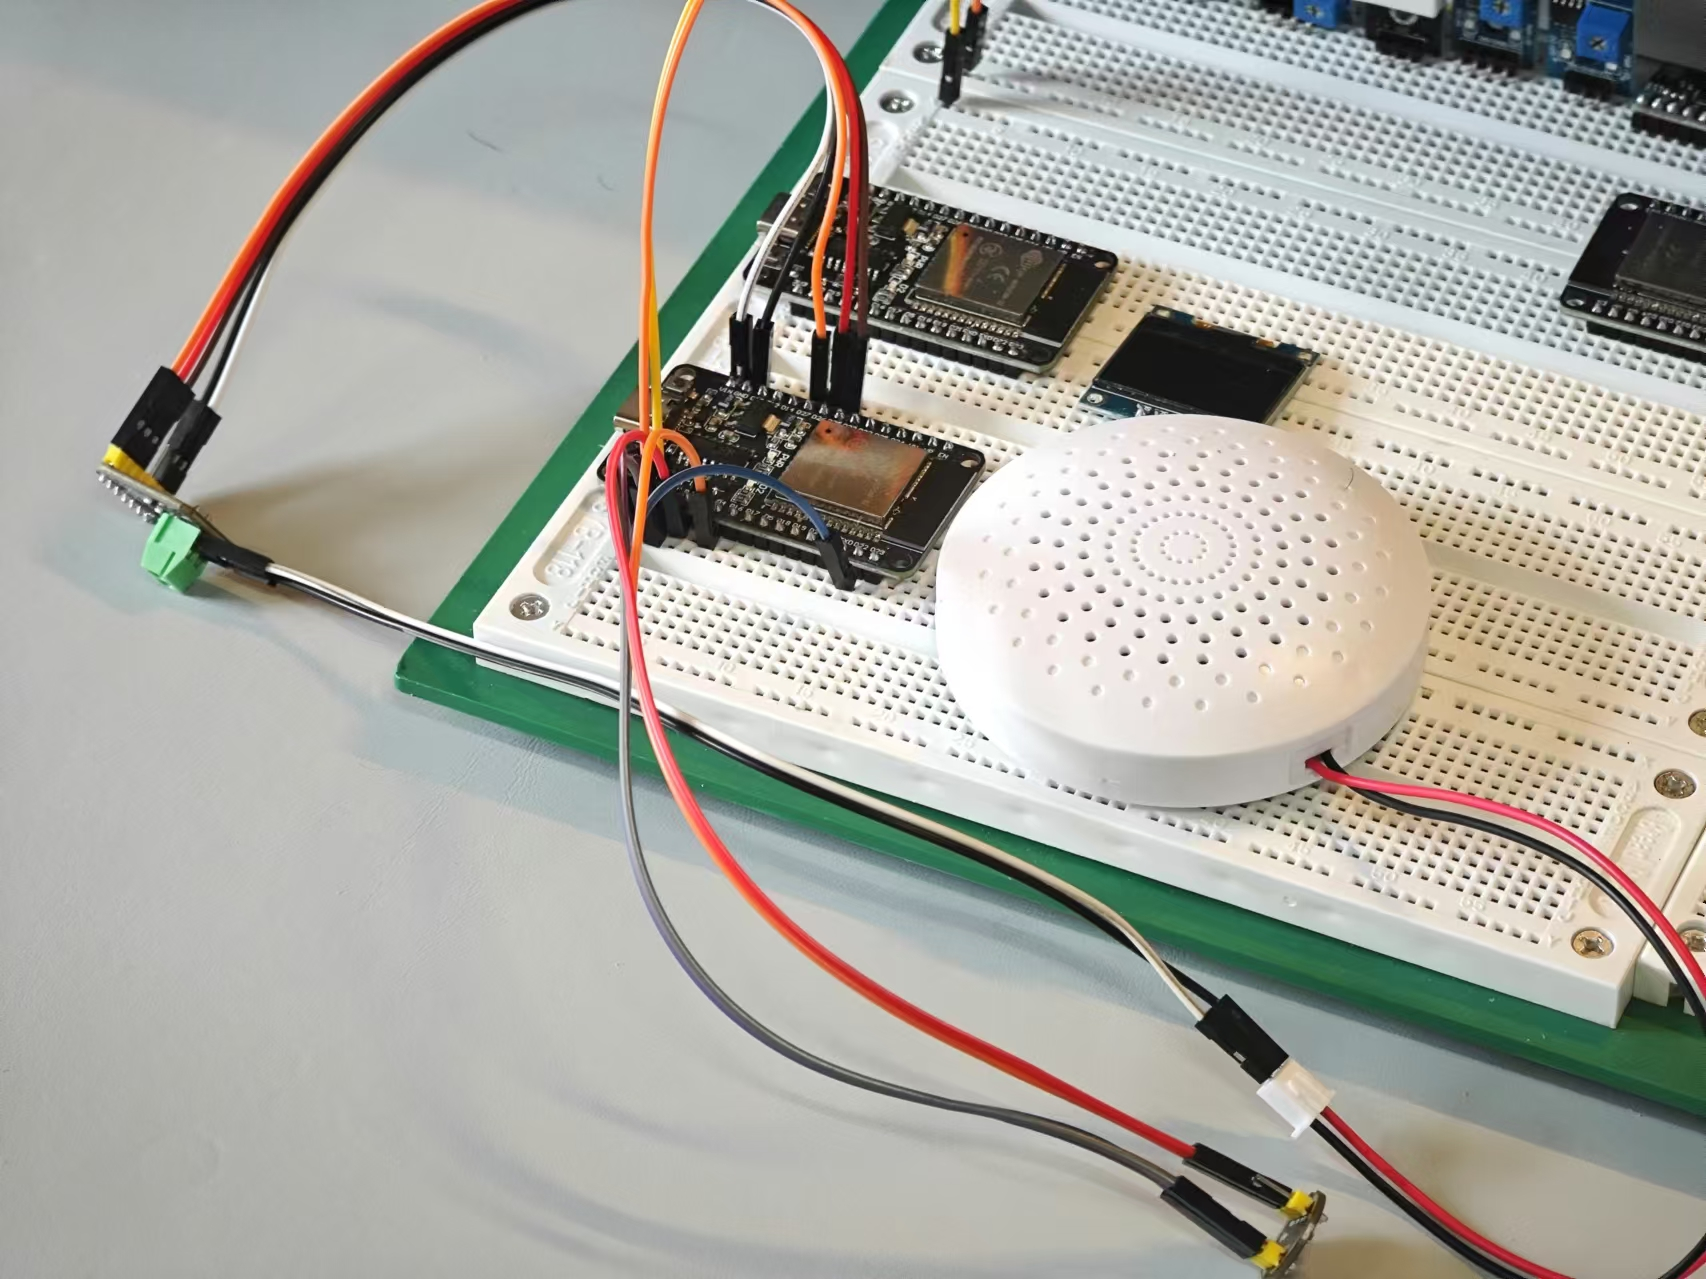
\includegraphics[width=0.4\textwidth]{../img/MasterConn.jpg}
    \caption{主机(Master)接线图}
\end{figure}

\subsection{从机(Slave)接线表如下}

\begin{table} [H]
    \centering
    \begin{tabular}{|c|c|c|l|}
    \hline
    \textbf{引脚编号} & \textbf{引脚名称} & \textbf{接入点} & \textbf{功能/用途} \\ 
    \hline
    1  & 3V3   & 面包板长线 & 提供3.3V电压输出 \\ 
    2  & GND   & 面包板长线 & 接地 \\ 
    4  & GPIO36  & MQ5 AO  & 获取MQ5模拟信号 \\ 
    5  & GPIO25  & DHT22 Output  & 获取DHT22数据 \\ 
    6  & GPIO33   &  Raindrop Module   & 获取雨量数据 \\
    7  & GPIO32   &  MQ135 Module   & 获取有毒气体数据 \\
    8  & GPIO35   &  MQ135 Module   & 获取有毒气体数据 \\
    9  & GPIO34   &  Light Module   & 获取光照强度数据 \\
    10  & GPIO36   &  Fire Module   & 获取火焰传感器数据 \\
    \hline
    \end{tabular}
    \caption{ESP32 引脚接线表}
\end{table}

\begin{figure} [H]
    \centering
    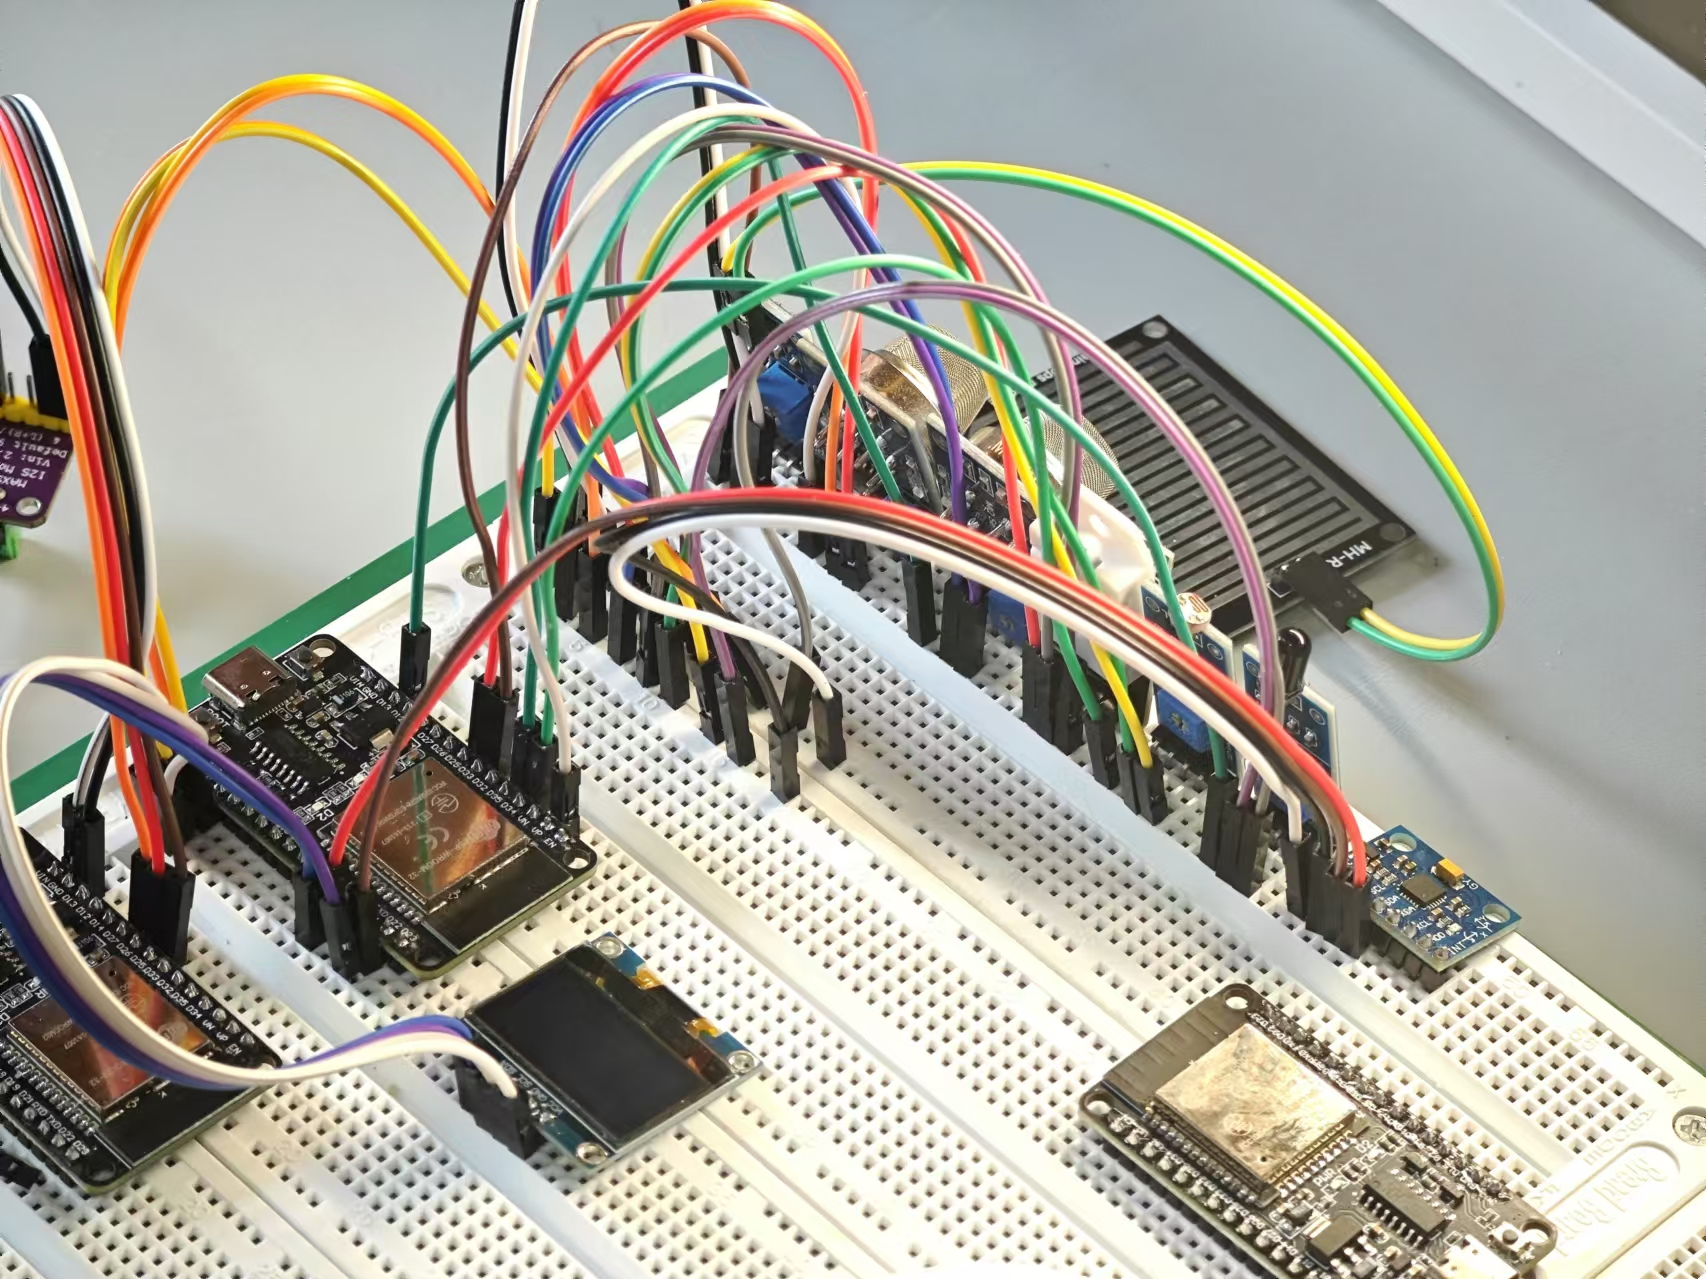
\includegraphics[width=0.4\textwidth]{../img/SlaveConn.jpg}
    \caption{从机(Slave)接线图}
\end{figure}

\end{document}